\section{ВЫДЕЛЯЕМЫЕ ИНТЕНТЫ}
Прежде чем приступать к созданию набора данных, необходимо определить список намерений (интентов), которые система должна различать. 
При этом важно учитывать уровень взаимодействия игрока и неигровых персонажей (далее NPC): игрок может ожидать от NPC не только 
словесного ответа, но и каких-то действий, будь то торговля, обмен, перемещение NPC и т.д. 
Помимо этого, если игрок хочет просто поговорить, для формирования более корректного ответа важно понимать, что именно игрок говорит NPC: 
это приветствие, вопрос, касающийся знаний NPC о чём-то, и т.п.

Таким образом интенты можно разделить на две основные группы:
\begin{enumerate}
   \item Интенты для взаимодействия с игровой механикой;
   \item Интенты для более полного понимания диалога игрока с NPC.
\end{enumerate}
\subsection{Интенты для взаимодействия с игрой}
Перед составлением списка интентов, предполагающих взаимодействие с игрой, надо выделить универсальный для наибольшего количества игр
набор действий, которые может совершить NPC в ответ на реплику игрока. Проведя некоторое исследование, было решено выделить следующие действия:
\begin{itemize}
   \item Обмен или торговля (данные действия было решено не разделять, так как из реплики далеко не всегда может быть понятно, что именно хотел игрок);
   \item Нападение на других NPC;
   \item Перемещение NPC;
   \item Защита игрока, места или другого NPC;
   \item Передача устного сообщения;
   \item Следование за игроком или другим NPC;
   \item Стать напарником/помощником игрока;
   \item Передача предмета другому NPC;
   \item Выдача задания игроку;
   \item Завершение выполненного игроком задания;
   \item Реакция на угрозу от игрока (это может быть нападение NPC на игрока, паническое бегство или что-то ещё).
\end{itemize}
Каждому действию был присвоен соответствуюищй интент.
\subsection{Интенты для понимания фраз игрока в диалоге}
Для более корректной генерации ответа на фразу игрока были выделены следующие интенты:
\begin{itemize}
   \item Приветствие (для ответа на привествие со стороны игрока приветствием со стороны NPC);
   \item Вопрос, предполагающий наличие знаний NPC о других NPC или о мире игры в целом (для поиска контекста для модели генерации ответа в общей системе);
   \item Обычные фразы, не предполагающие наличие специальных знаний (например <<Что делаешь?>>, <<Как дела?>> и т.п.);
   \item Шутка (ответом на шутку может быть как смех, так и непонимание со стороны NPC);
   \item Бессмысленный набор букв или слов (ответ NPC предполагает непонимание фразы);
   \item Прощание (для ответа на прощание прощанием и передачи информации игре о завершении диалога).
\end{itemize}

\section{ГЕНЕРАЦИЯ ДАННЫХ}
Для получения основного корпуса данных был использован метод маскирования, часто использующийся для аугментации данных в задаче распознавания имён сущностей (Name Entity Recognition или NER). При использовании такого метода примеры в наборе данных получаются несколько однообразные, поэтому в дополнение к данным, полученным с помощью маскирования, добавляются данные, полученные с помощью модели перефразирования.

Так как метод маскирования позволяет сгенерировать очень большое количество примеров, было принято решение получить как можно больше таких данных, затем перемешать примеры, часть из них перефразировать с помощью модели, затем выбрать из перефразированных и изначальных примеров случайным образом некоторый набор данных в пропорции 1 к 1 (иногда из-за особенностей некоторых интентов пропорции смещались в ту или иную сторону). Таким образом, в итоговом наборе будут как более качественные примеры, полученные методом маскирования, так и менее качественные, полученные с помощью модели перефразирования.

Примеры для классификации бессмысленных запросов генерировались отдельно следующим образом: был создан набор слов и последовательностей 
символов, а из них случайным образом создавалась последовательность от 1 до 25 слов.

Важно заметить, что примеры для интента <<Шутка>> были взяты из открытых источников. Это связано с тем, что 
изменение шутки методом маскирования или перефразированием может исказить её смысл настолько, что шутка перестанет быть шуткой.

Ещё одним интентом, для которого данные не генерировались, является интент, обозначащий фразы игрока, 
не предполагающие наличие специальных знаний. Примеры для этого класса были взяты также из открытых источников, так как генерация таких 
примеров сложнее, а в открытых источниках имеются нужные данные.

\subsection{Метод маскирования}
Метод маскирования заключается в следующем: 
\begin{enumerate}
    \item Выбирается несколько примеров для аугментации;
    \item Выбранные сущности в них заменяются специальным набором символов, т.е. маской (например, \texttt{[ITEM]});
    \item Выбирается набор сущностей, которые могут находится в примерах на месте маски;
    \item В каждый пример вместо маски подставляются всевозможные варианты сущностей.
\end{enumerate}

Для генерации изначального набора примеров и сущностей была использована инструкционная модель от OpenAssistant. Кроме того, большое количество 
сущностей было получено переводом простых слов (яблоко, хлеб, меч, брюки, человек, торговец и т.п.) на английский язык.

Важно учитывать тот факт, что если подставлять вместо маски любые сущности или наборы сущностей, можно получить большое количество 
неадекватных примеров, например, <<Я хочу купить 2150 мечей>> и т.п. 

\subsection{Модель перефразирования}
В настоящее время существует множество сервисов для перефразирования текста, однако все или почти все из них либо являются платными, 
либо имеют  очень ограниченный бесплатный тарифный план, что не позволяет использовать их для перефразирования большого количества примеров. 
В связи с этим было принято решение использовать предобученную модель с HuggingFace. В качестве такой модели была выбрана модель 
\texttt{chatgpt\_paraphraser\_on\_T5\_base}. Это базовая модель T5, дообученная на датасете перефразирования, сгенерированном с помощью 
\texttt{ChatGPT}. Такой выбор связан с тем, что остальные модели, представленные на HuggingFace для этой задачи, оказались слишком слабыми: 
либо не меняли предложение, либо слишком сильно искажали изначальный смысл.

После проведения нескольких экспериментов был выбран наиболее удачный набор параметров (таблица \ref{tab1:table}).

\begin{table}[H]
   \captionsetup{format=hang, singlelinecheck=false}
   \raggedleft
      \caption{Параметры генерации для модели перефразирования}
      \label{tab1:table}
   \centering        
   \begin{tabular}{|p{10cm}|p{5cm}|}
      \hline
      num\_beams & 5 \\
      \hline
      num\_beams\_groups & 5 \\
      \hline
      num\_return\_sentences & 5 \\
      \hline
      repetition\_penalty & 10.0 \\
      \hline
      diversity\_penalty & 3.0 \\
      \hline
      no\_repeat\_ngram\_size & 2 \\
      \hline
      temperature & 0.7 \\
      \hline
      max\_length & 512 \\
      \hline
   \end{tabular}
\end{table}

\section{ОБРАБОТКА И АНАЛИЗ ПОЛУЧЕННЫХ ДАННЫХ}
В процессе генерации данных было обнаружено, что в некоторых ситуациях модель перефразирования текста может добавлять в примеры лишние символы, 
слова и целые фразы, что связано с датасетом, на котором она обучена. Например, модель может добавить ещё один или несколько дополнительных 
знаков препинания, кавычки, какую-то дополнительную информацию в скобках и т.п. Наличие таких ошибок в заметном количестве может сказаться на 
качестве итоговой модели, поэтому было решено избавиться от них.

Так как данные генерировались по классам, следующий этап предобработки заключается в объединении сгенерированных данных в единый набор и разделение на подвыборки для обучения, валидации и тестирования моделей. Для того, чтобы данные на разных подвыборках не сильно отличались друг от друга и в каждой подбвыборке распределение по классам было одинаковое, разделение происходило следующим образом:
\begin{enumerate}
   \item Данные по каждому классу загружались отдельно и перемешивались;
   \item Затем данные по каждому классу разделялись на разные подвыборки (8:1:1 на тренировку, валидацию и тестирование);
   \item После данные объединялись по подвыборкам и каждая из них перемешивалась. 
\end{enumerate}

После объединения был проведён анализ полученных данных. Общий размер набора данных примерно 2,2 миллиона токенов или 163,2 тысячи 
примеров. Средняя длина одного примера 13 токенов. 
В среднем количество примеров по каждому классу составляет около 10000 примеров (рисунок \ref{classnumbers:image}). 
Однако количество примеров по некоторым классам меньше 10000 (от 4000 до 7000), что связано со сложностью создания примеров для 
этих классов.
\begin{figure}[H]
   \begin{center}
      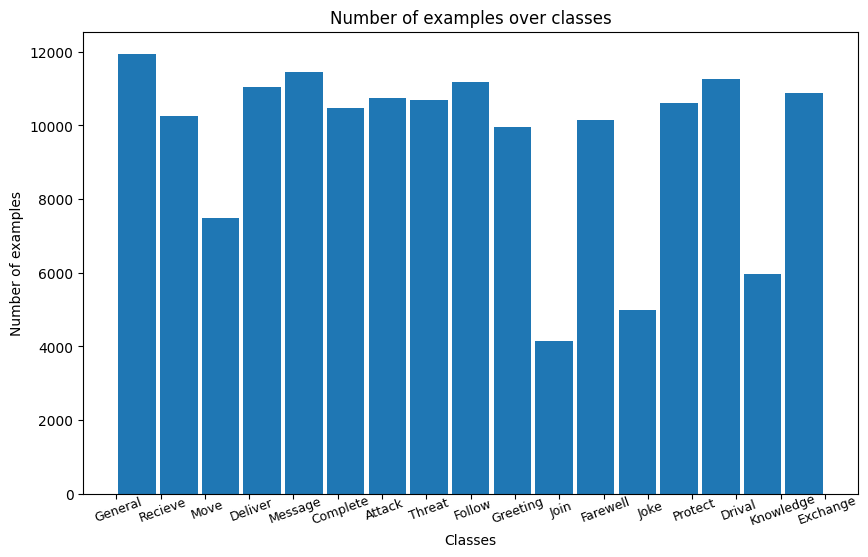
\includegraphics[width=.7\linewidth]{examples_over_classes.png}
      \caption{Распределение примеров по классам}
      \label{classnumbers:image}
   \end{center}
\end{figure}

Кроме того, набор имеет следующее распределение длин примеров в токенах (рисунок \ref{tokennumbers:image}).
\begin{figure}[H]
   \begin{center}
      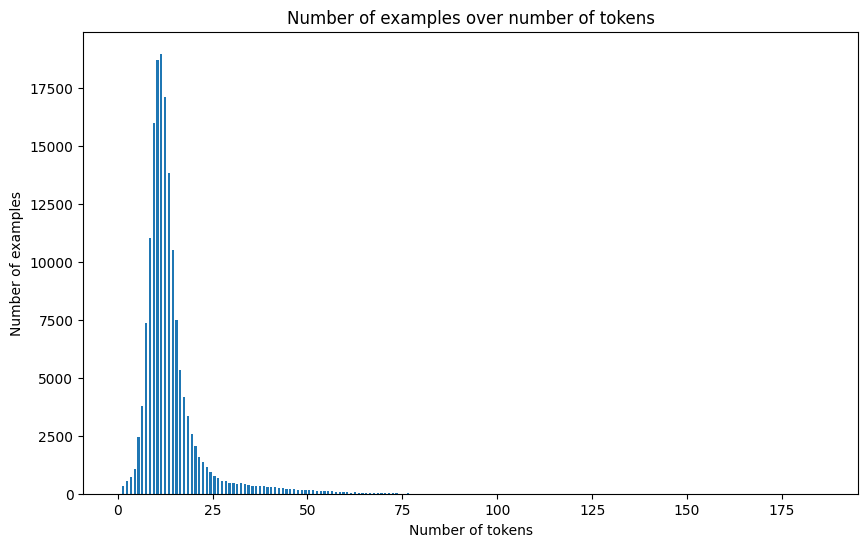
\includegraphics[width=.7\linewidth]{examples_over_tokens.png}
      \caption{Распределение примеров по количеству токенов}
      \label{tokennumbers:image}
   \end{center}
\end{figure}

Далее приведено несколько примеров из полученного набора данных (таблица \ref{examples:table}).
\begin{table}[H]
   \captionsetup{format=hang, singlelinecheck=false}
   \raggedleft
      \caption{Примеры из полученного набора данных}
      \label{examples:table}
   \centering        
   \begin{tabular}{|p{11cm}|p{5cm}|}
      \hline
      Примеры & Классы примеров \\
      \hline
      Your task is to hand saber to Annah. & Deliver \\
      \hline
      Hello, dear friends! & Greeting \\
      \hline
      tomorrow one integer hundred claim Follow elves drop man & Drival \\
      \hline
      Make sure you choose wisely, because every move counts, Beithira Soulforger! & Threat \\
      \hline
      I'd like to sell tomato, steak. & Exchange \\
      \hline
      I would like to buy pike and falchion. & Exchange \\
      \hline
      Could you come after Kieran Fireblood? & Follow \\
      \hline
      I want you to beat that bandit. & Attack \\
      \hline
      Are you capable of killing Annah? & Attack \\
      \hline
      You are responsible for safeguarding an outpost. & Protect \\
      \hline
      Please, go to this wayfarer. & Move \\
      \hline
      What can you tell me about Caravan Crossroads? & Knowledge \\
      \hline
      We will never speak again, Adira Whitesnow. & Farewell \\
      \hline
      Please take care Brianna Moonlight. & Farewell \\
      \hline
      Join me. & Join \\
      \hline
      i don't know. & General \\
      \hline
      Why does lightning always strike trees? They are the path of leaf resistance. & Joke \\
      \hline
      Can i find mission for me in Goldgrasp? & Recieve quest \\
      \hline
      May I ask you to communicate with Hargrimm the Bleak. & Message \\
      \hline
      I've completed your job in Deeproot Village. & Complete quest \\
      \hline
   \end{tabular}
\end{table}